\documentclass[a4paper,12pt]{scrbook} 

\usepackage[utf8]{inputenc} 
\usepackage[T1]{fontenc}
\usepackage[ngerman]{babel}

%Das Paket wird für die anderthalb-zeiligen Zeilenabstand benötigt
\usepackage{setspace}


%%HTWM-Vorlage - benoetigt apt-get install texlive-fonts-extra
\setcounter{tocdepth}{2}				%Schatelungstiefe Inhaltsverz.

\usepackage[hyphens]{url} %lange URLs werden damit am Zeilenende umgebrochen
\usepackage[utf8]{inputenc}			%deutsche Umlaute
\usepackage{german, ngerman}
\usepackage[ngerman]{babel}		%Rechtschreibprüfung
\usepackage{color,listings} %Quellcode Highlighting, bindet das
\usepackage{float}					%% GRAFIKPOSITION MITTELS [H] ERWZINGEN
%Paket Listings ein
%%
\usepackage{color}
\usepackage{textcomp}
\usepackage[T1]{fontenc}				%srccode
\usepackage[scaled]{beramono}		%srccode
\usepackage{longtable}				%mehrseitige tabellen
\usepackage[tableposition=b]{caption}
\usepackage[pdftex, pdftoolbar=false, hyperfootnotes=false,bookmarks,bookmarksopen, bookmarksnumbered, bookmarksopenlevel=2,pdfpagelabels=true,pdfstartpage=1,pdfstartview=FitH]{hyperref} %PDF-Verlinkungen
\usepackage{array}					%farbige Tabellen
\usepackage[table]{xcolor} 			%farbige Tabellen
\usepackage{graphicx}				% \includegraphics bnoetigt dies

\usepackage{fancyhdr, graphicx}	

\usepackage{amsmath}
\usepackage{amsthm}
\usepackage{amsbsy}
\usepackage{amssymb}


\usepackage{float} %% force image position by using big H: \begin{figure}[H]
\usepackage{datetime} %% \today zusaetzlich mit uhrzeit

\usepackage{menukeys}

\definecolor{Navy}{rgb}{0,0,0.5}
\definecolor{Gray}{gray}{0.5}
\definecolor{dunkelgrau}{rgb}{0.8,0.8,0.8}
\definecolor{hellgrau}{rgb}{0.95,0.95,0.95}
\definecolor{hellgrau2}{rgb}{0.93,0.93,0.93}
\definecolor{listinggray}{gray}{0.9}
\definecolor{lbcolor}{rgb}{0.9,0.9,0.9}

\hypersetup{
	colorlinks=true, 			% false: boxed links; true: colored links
	linkcolor=Navy,          		% color of internal links
	citecolor=Gray,        			% color of links to bibliography
	filecolor=magenta,      		% color of file links
	urlcolor=blue,           			% color of external links
	linkbordercolor={1 1 1}, 		% set to white
	citebordercolor={1 1 1} 		% set to white
}


%Einrückung eines neuen Absatzes
\setlength{\parindent}{0em}

%Definition der Ränder
\usepackage[paper=a4paper,left=30mm,right=30mm,top=30mm,bottom=30mm]{geometry}

%Abstand der Fussnoten
\deffootnote{1em}{1em}{\textsuperscript{\thefootnotemark\ }}

\begin{document}

\begin{titlepage}

\begin{figure}[H]
\begin{center}
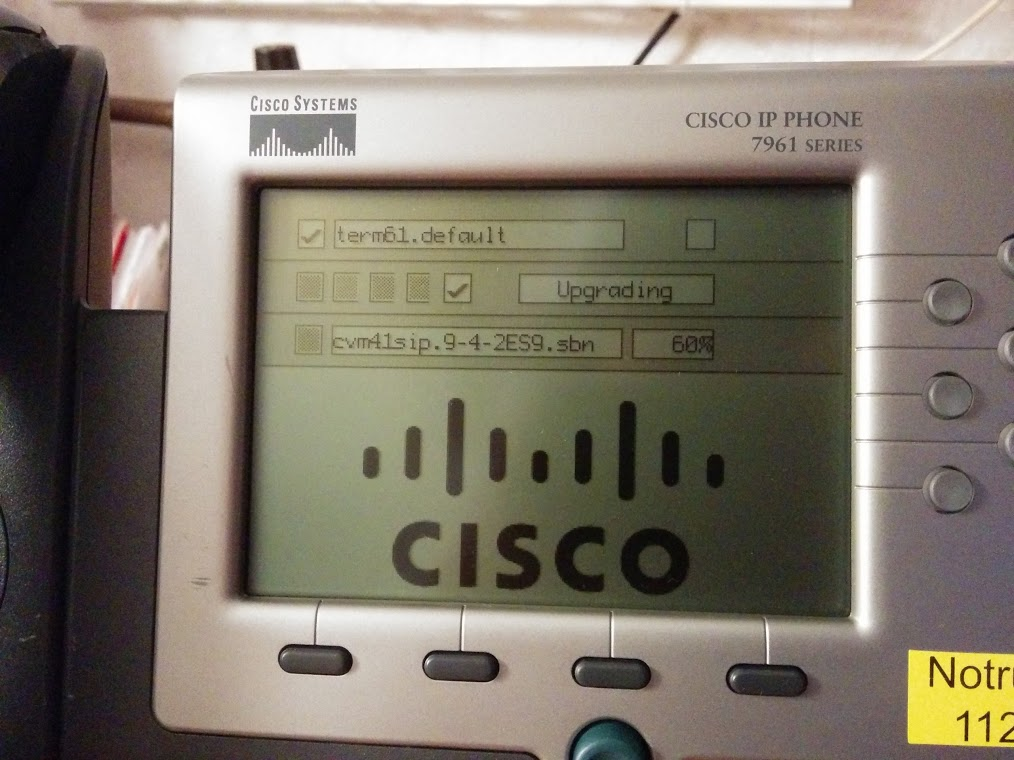
\includegraphics[width=.7\hsize]{./images/ciscoupdate.jpg}
\end{center}
\end{figure}


\begin{center}
{\huge\bfseries VoIP-Setup: FritzBox 7240 am Telekom AllIP-DSL mit Cisco 7960,7961,7962 Systemtelefonen verheiraten\par}
\vskip 1cm
\textbf{Beispielkonfiguration}

WARNUNG: Ich bin nicht verantwortlich wenn ihr bei dem Versuch das nachzustellen eure Hardware in Briefbeschwerer verwandelt. Ich
beschreibe hier nur nach bestem Wissen und Gewissen, wie es bei mir geklappt hat. Wie immer gilt:\\
\textbf{Gehirn einschalten, nachmachen auf eigene Gefahr !!}\\
HINWEIS ZU FIRMWARE-/BIOS UPDATES IM ALLGEMEINEN: Bei einem Firmware-/BIOS-Update die Geduld zu verlieren und den Stecker zu ziehen,
weil sich mal 10 Minuten nichts regt, ist der sicherste Weg eure Hardware kaputt zu machen ! Im Zweifel über Nacht stehen lassen, wenn
sich bis zum nächsten Morgen immernoch nichts getan hat, kann man immernoch neustarten. Beispielsweise laufen die Cisco 7961 mit Java und
brauchen locker mal eine halbe Stunde, wenn man die SIP-Firmware updatet. 
\end{center} 
\vfill
%%\vskip 3cm
\flushleft
\begin{tabular}{rl}
Autor: & marcel\\ 
Version: & v0.2\\
Am: & \today\\
HINWEIS: &Fast alles in dieser Anleitung stammt aus dem Netz, ich hab es nur so\\ &zusammengefummelt, das es für mich funktioniert.\\
\end{tabular}
\end{titlepage}

%Inhaltsverzeichnis (aktualisiert sich erst nach dem zweiten Setzen)
\tableofcontents

%Abbildungsverzeichnis und Tabellenverzeichnis auf einer Seite
%%\clearpage
\listoffigures


%%\listoftables	%% tabellnverzeichnis

%% 											\renewcommand{\lstlistlistingname}{Quellcodeverzeichnis}
\lstlistoflistings

%%  \thispagestyle{empty}
 
%Beginn einer neuen Seite
\clearpage
 
%Anderthalbzeiliger Zeilenabstand ab hier
\onehalfspacing
 
 %% ab hier Bilder mit Abb. statt Abbildung beschriften
 \renewcommand{\figurename}{Abb.}

%% Syntax Highlighting für BASH
\lstset{
	language=XML,
	keywordstyle=\bfseries\ttfamily\color[rgb]{0,0,1},
	identifierstyle=\ttfamily,
	commentstyle=\color[rgb]{0.133,0.545,0.133},
	stringstyle=\ttfamily\color[rgb]{0.627,0.126,0.941},
	showstringspaces=false,
	basicstyle=\scriptsize,
	tabsize=1,
	numbers=left,                    % where to put the line-numbers; possible values are (none, left, right)
	numbersep=5pt,                   % how far the line-numbers are from the code
	numberstyle=\tiny\color{gray}, % the style that is used for the line-numbers
	breaklines=true,	%automatischer Zeilenumbruch
	prebreak =\raisebox{0ex}[0ex][0ex]{\ensuremath{\hookleftarrow}},
	breakatwhitespace=false,
	aboveskip={1.5\baselineskip},
  	columns=fixed,
  	upquote=true,
  	extendedchars=true,
  	backgroundcolor=\color[rgb]{0.97,0.97,0.97},
}


%\pagestyle{plain}
\pagestyle{fancy}

\pagestyle{fancy} 
\fancyhf{}  % Kopf- und Fußzeile leeren 
\renewcommand{\headrulewidth}{1pt} 
\fancyhead[EL]{\nouppercase{\leftmark}} %Kopfzeile linker Bereich auf geraden Seiten
\fancyhead[OR]{\nouppercase{\leftmark}} %Kopfzeile rechter Bereich auf ungeraden Seiten
\fancyfoot[EL]{\thepage} %% Seitenzahl links auf geraden Seiten
\fancyfoot[OR]{\thepage} %% Seitenzahl rechts auf ungeraden Seiten



\clearpage
\chapter{Einleitung}
\label{sec:0}
Dieses Dokument beschreibt mein privates Telefoniesetup zu Hause. Da es mich ein wenig Zeit gekostet hat die einzelnen Komponenten
so zum Zusammenspiel zu bewegen, möchte ich den Weg hiermit dokumentieren.

WARNUNG: Ich bin nicht verantwortlich wenn ihr bei dem Versuch das nachzustellen eure Hardware in Briefbeschwerer verwandelt. Ich
beschreibe hier nur nach bestem Wissen und Gewissen, wie es bei mir geklappt hat. Wie immer gilt: 


\textbf{Gehirn einschalten, nachmachen auf eigene Gefahr !!}


HINWEIS ZU FIRMWARE-/BIOS UPDATES IM ALLGEMEINEN: Bei einem Firmware-/BIOS-Update die Geduld zu verlieren und den Stecker zu ziehen,
weil sich mal 10 Minuten nichts regt, ist der sicherste Weg eure Hardware kaputt zu machen ! Im Zweifel über Nacht stehen lassen, wenn
sich bis zum nächsten Morgen immernoch nichts getan hat, kann man immernoch neustarten. Beispielsweise laufen die Cisco 7961 mit Java und
brauchen locker mal eine halbe Stunde, wenn man die SIP-Firmware updatet. 


\chapter{Hardware}
\label{sec:1}

Die eingesetzte Hardware untergliedert sich in drei Kathegorien und setzt sich wie folgt zusammen:

\begin{itemize}
 \item Router (stellt DSL-Verbindung her und dient als DHCP-Server für das LAN):
 \begin{itemize}
  \item IGEL UD3-H700C mit Intel Dual Gigabit Netzwerkkarte, daran Allnet ALL0333C DSL-Modem, Software: pfSense
 \end{itemize}
 \item VoIP-Server: 
 \begin{itemize}
  \item ausgediente FritzBox 7240 (DSL-Modem und WLAN defekt, Telefonieteil augenscheinlich noch funktionstüchtig)
 \end{itemize}
 \item VoIP:-Endgeräte:
 \begin{itemize}
  \item 1x LG Nexus 5 nativer Android VoIP Client
  \item 1x Siemens S685IP VoIP-DECT Basisstation
  \item 1x Cisco 7960 Systemtelefon mit SIP-Firmware
  \item 4x Cisco 7961 Systemtelefon mit SIP-Firmware
  \item 2x Cisco 7962 Systemtelefon mit SIP-Firmware (warte da derzeit noch auf die Warenlieferung)
 \end{itemize}
\end{itemize}

\section{Router}
Als Router setze ich einen Thinclient von Igel ein. Das verwendete Modell UH3-H700C hat keine bewglichen Teile, 
man kann sowohl CF-Karten als auch 2,5``-IDE-Platten verbauen und das wichtigste: es gibt einen vollwertigen PCI-Steckplatz.
In diesem sitzt eine Intel Dual-Gigabit Netzwerkkarte. Beide Komponenten habe ich sehr günstig (jeweils unter 20 Euro) beim
Auktionshaus meines Vertrauens erstanden. Der Igel kommt mit einem 12V Netzteil und sollte nicht signifikant mehr Energie
verbrauchen als andere Router

Als Software setze ich pfSense ein, eine Router-Distribution auf Basis von FreeBSD. pfSense selbst bietet extrem viele Möglichkeiten,
für mich interessant ist der sehr flexibel konfigurierbare DHCP-Server und vor allem lässt sich aus der Weboberfläche sehr leicht
ersehen welche lokale IP-Adresse gerade wieviel Internet-Bandbreite belegt - für schwachbrüstige DSL-Anschlüsse wie meinen ein, ein 
wesentliches Diagnosemittel. 

Der Igel macht bei mir wirklich nur die DSL-Einwahl, WLAN und VoIP beispielsweise machen bei mir separate Geräte, dazu später mehr.
Die Lösung Igel+pfSense setze ich jetzt seit Jahren ein und mein Fazit ist bisher: rockstable.

Weiterer wichtiger Punkt: die komplette Konfiguration lässt sich als XML-Datei exportieren.

\section{VoIP-Server}
Als VoIP-Server kann man prinzipiell neben Fertigprodukten wie beispielsweise von AVM oder Lancom auch selbst VoIP-Installationen aufsetzen.
Es gibt hierzu diverse Distributionen auf Basis von Asterisk wie beispielsweise die Distributionen AsteriskNow oder FreePBX. Aber das schien mir
für meine privaten Zwecke dann doch Overkill. Außerdem möchte ich da keinen großen Wartungsaufwand bei der Telefonanlage.

\subsection{Fritzbox 7240 als VoIP-Server}
Bei einem Bekannten konnte ich eine AVM FritzBox 7240 vor der Verschrottung retten, an der nach einem Gewitter das DSL-Modem sowie 
WLAN ausgefallen waren. Die FritzBox wird so konfiguriert das sie eine lokale IP-Adresse aus dem LAN erhält und das Internet über den
IGEL-Router mit benutzt. Am Igel sind die relevanten Ports für VoIP an die FritzBox weitergeleitet. Dazu später mehr.

Wie beim IGEL-Router auch, lässt sich auch bei der FritzBox die komplette Konfiguration als XML-Datei sichern.


\section{VoIP-Clients}
Das ganze Projekt ist aus dem Wunsch heraus entstanden, neben den Mobilteilen, die durch die Siemens S685IP versorgt werden auch wieder ein
''Festnetztelefon`` zur Verfügung zu haben. Über das Auktionshaus meiner Wahl bin ich dann auf das Cisco 7960 aufmerksam geworden. Zunächst
skeptisch ob der SCCP-Firmware, habe ich das Ding erstanden. Da es nach etwas Gefummel sowohl von der Haptik als auch von der Sprachqualität 
überzeugt hat, habe ich noch ein paar Nachfolgemodelle 7961 und 7962 erstanden. Wenn man den Konfigurations- und Updatevorgang einmal prinzipiell
verstanden hat, ist es trivial eine fast beliebige Anzahl weiterer solcher Modelle in Betrtieb zu nehmen. 

\chapter{Konfiguration}
In unserem Szenario haben wir folgende Geräte:
\begin{description}
 \item[IP 192.168.1.1]  IGEL-Router stell Internetverbindung her und dient als DHCP-Server
 \item[IP 192.168.1.2]  TFTP-Server der die Firmware- und Konfigurationsdateien vorhält (bei mir: Ubuntu mit atftpd)
 \item[IP 192.168.1.80] FritzBox als interner VoIP-Server
 \item[IP 192.168.1.91] Nexus 5 als VoIP Client mit interner Rufnummer 620 und Passwort 1234
 \item[IP 192.168.1.81] Siemens S685IP als VoIP Client mit interner Rufnummer 621 und Passwort 1234
 \item[IP 192.168.1.82] Cisco 7960 als VoIP Client mit interner Rufnummer 622 und Passwort 1234
 \item[IP 192.168.1.83] Cisco 7961 als VoIP Client mit interner Rufnummer 623 und Passwort 1234
\end{description}

\section{Router}
Am Router selbst ist nichts zu beachten, solange eine zuverlässige Internetverbindung besteht und die passenden Ports zum VoIP-Server durchgereicht werden.
Das sind in meinem Fall folgende Ports:
\begin{itemize}
 \item Ports 3478 bis 3480 TCP+UDP
 \item Ports 5060 bis 5080 UDP
 \item Ports 30000 bis 31000 UDP
 \item POrts 40000 bis 41000 UDP
\end{itemize}

Diese Ports muss man per NAT zur lokalen IP-Adresse des VoIP-Servers durchreichen.

Falls man pfSense einsetzt, sollte man beim erstellen der Portregeln darauf achten, dass man 
unten bei ''filter rule association`` die Standardvorgabe in ''pass`` umändert. Weiterhin sollte man sich
dieses Dokument \footnote{\url{https://doc.pfsense.org/index.php/VoIP_Configuration}} verinnerlichen, da
beispielsweise mit der standardmäßig aktivierten Option ''source port randomization`` kein stabiler VoIP-Betrieb 
zu machen ist.

\section{VoIP-Server}
Am VoIP-Server, also der FritzBox gibt es nun zwei Bereiche die man abarbeiten muss. Ein Teil ist die Registrierung der externen SIP-Nummern,
die man von seinem Anbieter zur Verfügung gestellt bekommen hat. In meinem Fall handelt es sich um 3 SIP-Nummern an einem AllIP-Anschluss der Telekom.
Der zweite Bereich ist die Konfiguration der FritzBox als SIP-Server für die internen SIP-Telefone.


Netter Nebeneffekt wenn man die FritzBox als VoIP-Server verwendet: falls man ein GMail-Konto hat, kann man seine Kontakte vom GMail-Konto direkt in die FritzBox importieren.
\subsection{Externe SIP-Accounts}
Hier hat man mit der FritzBox und dem mitgelieferten Assistenten wirklich leichtes Spiel. Man klickt sich durch den Telefonieassistenten, indem man seinen 
VoIP-Anbieter auswählt und noch die passenden Zugangsdaten einträgt. Danach sollte die FritzBox die SIP-Nummern porblemlos registrieren können. Wenn alles geklappt hat,
sollte das bei euch in der Art aussehen:

\begin{figure}[H]
\begin{center}
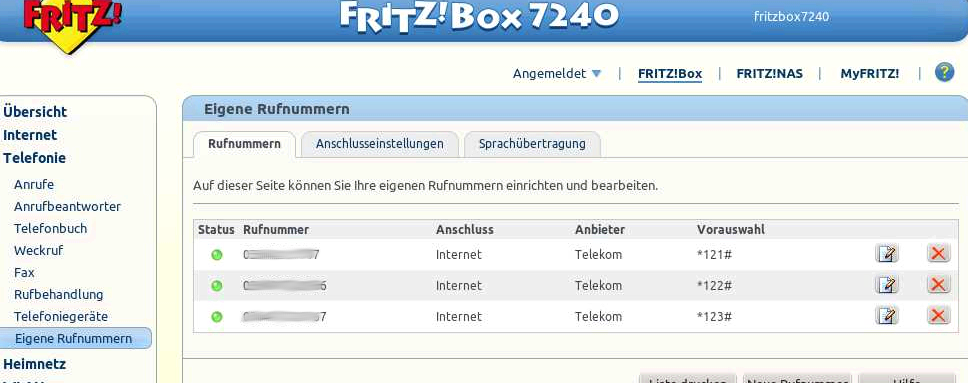
\includegraphics[width=1\hsize]{./images/voip-server-fritzbox-extsip.png}
\end{center}
\caption[Konfiguration externen SIP-Accounts, hier am Beispiel Telekom AllIP.]
{\label{voip-server-fritzbox-extsip}Konfiguration externen SIP-Accounts, hier am Beispiel Telekom AllIP. Quelle:Autor}
\end{figure}

\subsection{Interne SIP-Accounts}
Nun müssen wir noch für jedes interne Telefon einen SIP-Account anlegen. Das ist ebenso einfach wie im vorherigen Schritt. Man fügt in der Weboberfläche 
der FritzBox neue Telefoniegeräte hinzu. Diese bekommen standardmäßig die Nummern 610 und aufsteigend zugewiesen. 

\begin{figure}[H]
\begin{center}
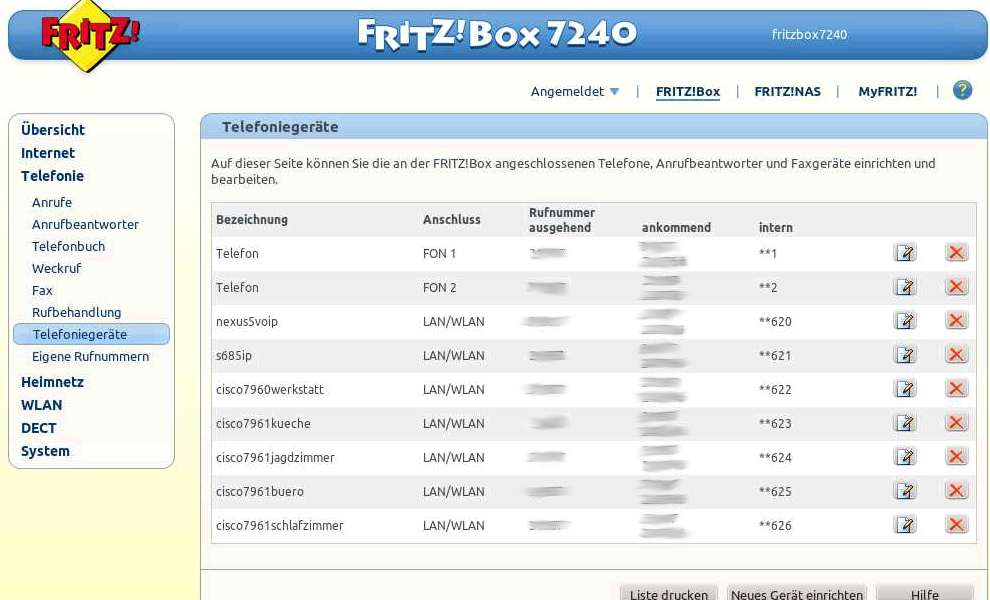
\includegraphics[width=1\hsize]{./images/voip-server-fritzbox-telefoniegeraete.png}
\end{center}
\caption[Konfiguration von SIP-Accounts für die internen Telefone.]
{\label{voip-server-fritzbox-intsip}Konfiguration von SIP-Accounts für die internen Telefone. Quelle:Autor}
\end{figure}

Als Passwort empfiehlt sich für die Testphase etwas 
unkompliziertes wie 1234 zu wählen, da einige ältere Telefone sich unter Umständen nicht an der FritzBox anmelden können, falls das Passwort zu komplex ist.
Solche Probleme sind dann nur sehr schwer zu diagnostizieren. Im letzten Schritt, wenn alles so läuft wie gewünscht, sollte man natürlich sämtliche Passwörter
durch sichere Passwörter ersetzen.

\begin{figure}[H]
\begin{center}
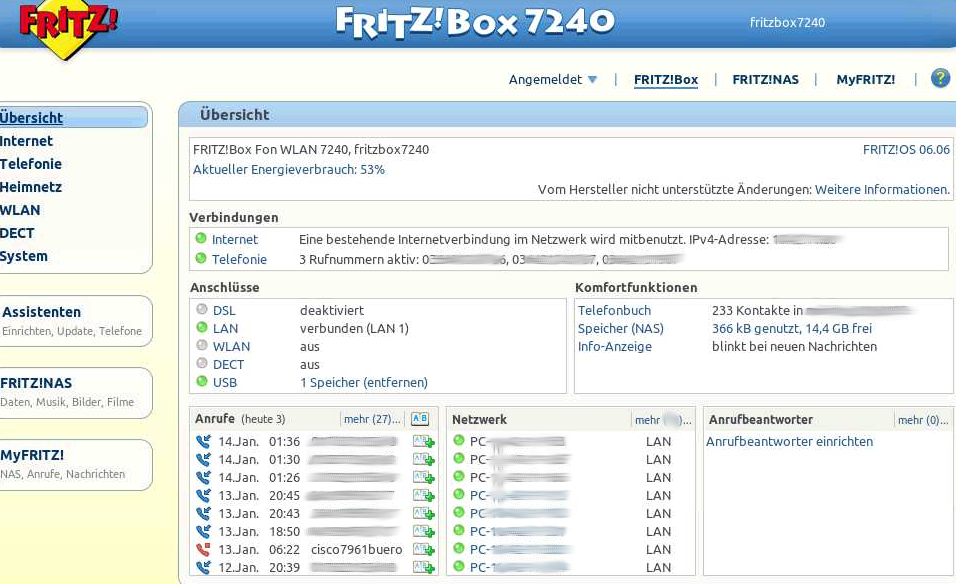
\includegraphics[width=1\hsize]{./images/voip-server-fritzbox-status.png}
\end{center}
\caption[FritzBox 7240 Konfiguration abgeschlossen und alle Nummern registriert.]
{\label{voip-server-fritzbox-status}FritzBox 7240 Konfiguration abgeschlossen und alle Nummern registriert. Quelle:Autor}
\end{figure}


\section{VoIP-Clients}
In diesem Kapitel beschreibe ich die Konfiguration meiner VoIP-Endgeräte im Haushalt, die sich dann an der FritzBox per SIP anmelden. Ich empfehle im LAN nur mit statischen
IP-Adressen zu arbeiten und sich nicht blind auf das lokale DNS zu verlassen. Zusätzlich hinterlege ich im IGEL-Router noch für die jeweilige MAC-Adresse eines Geräte die 
IP im DHCP-Server. So kann man die Geräte auch per DHCP konfigurieren lassen und es kommt trotzdem nicht zu IP-Problemen.

\subsection{LG Nexus 5}
Google's Betriebssystem Android bringt seit Version 4.2 einen nativen SIP-Client mit. Dieser eignet sich gut für erste Tests. Das zugehörige Optionsmenü ist jedoch sehr versteckt.
Man geht über die Telefon-App $\rightarrow$ Einstellungen $\rightarrow$ Anrufe $\rightarrow$ Anrufkonten $\rightarrow$ SIP-Konten.

Nun fügt man einen neuen SIP-Account hinzu:
\begin{itemize}
 \item Nutzername: 620
 \item Passwort: 1234
 \item Server: 192.168.1.80
\end{itemize}

\begin{figure}[H]
\begin{center}
%\includegraphics[width=.5\hsize]{./images/informationweek-virtualizationbycathegory.png}
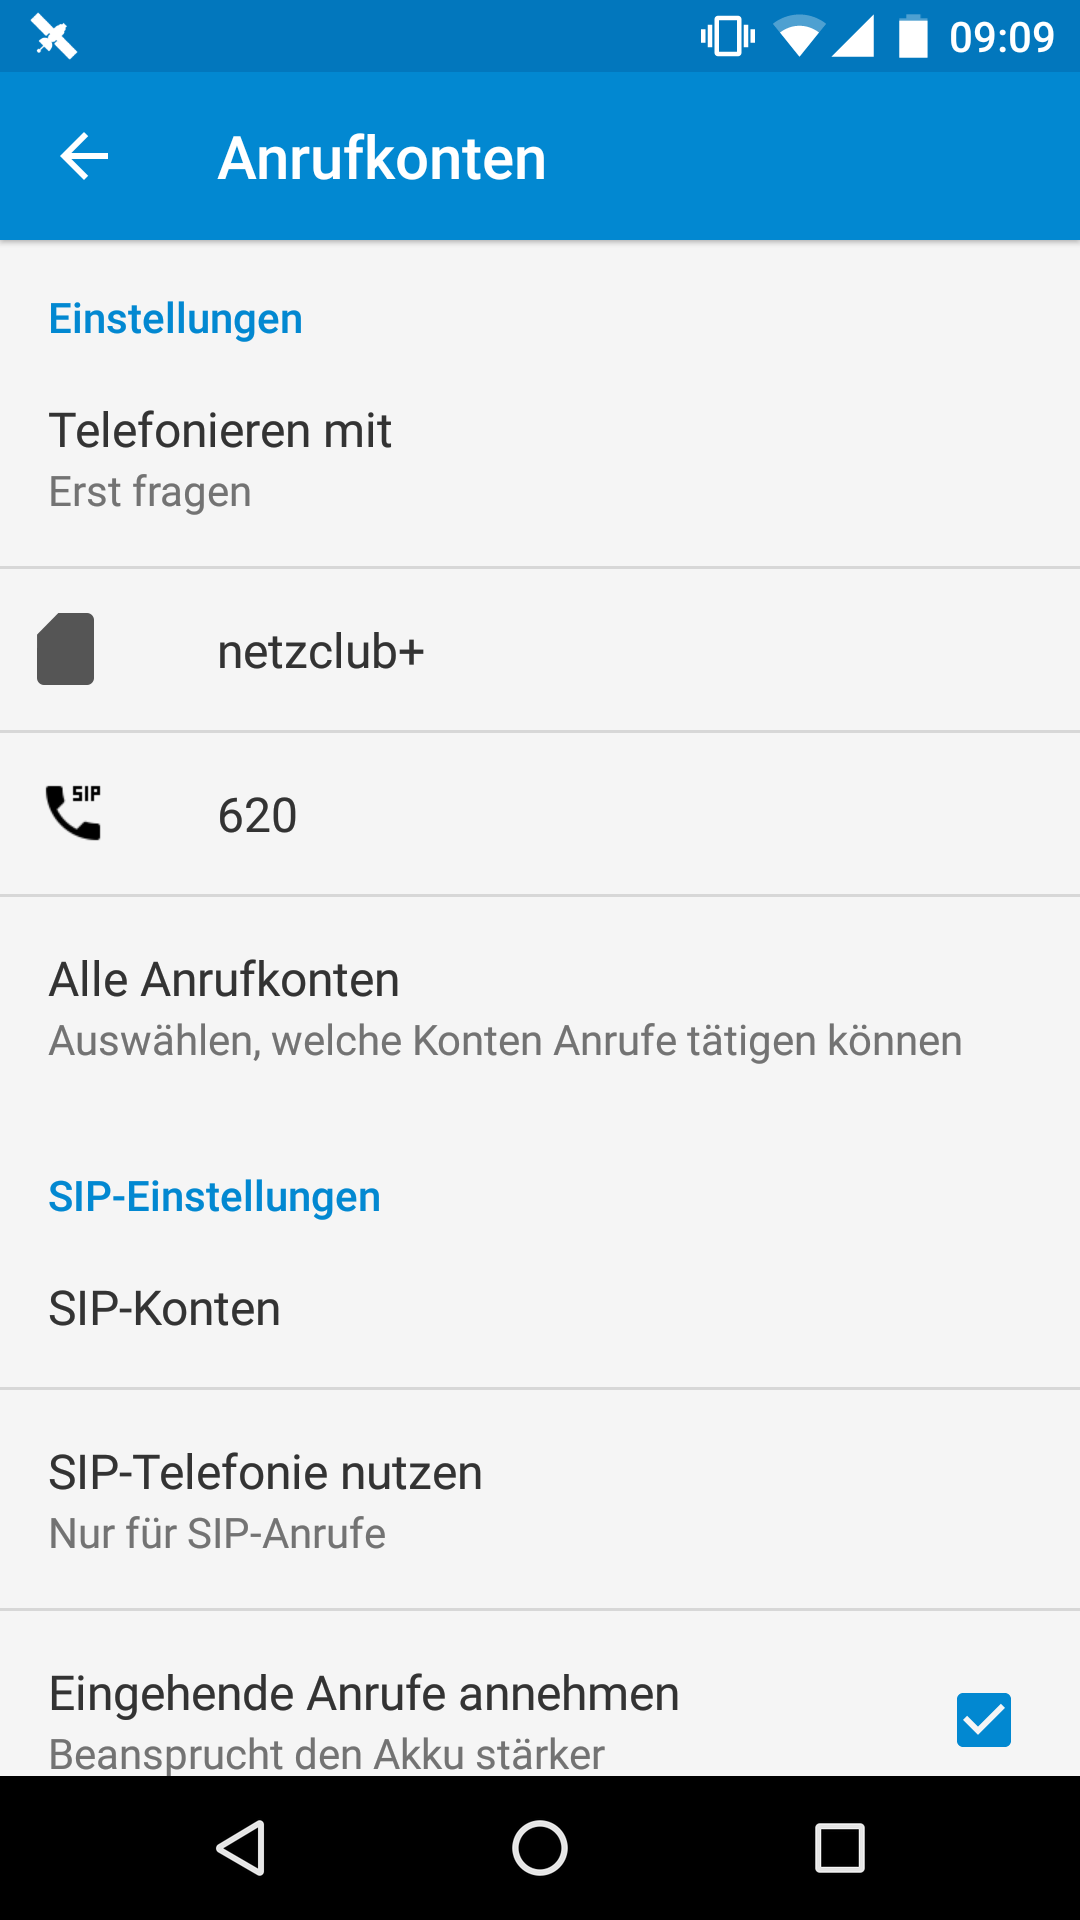
\includegraphics[width=.4\hsize]{./images/voip-client-nexus5.png}
\end{center}
\caption[Konfiguration eines SIP-Accounts in Android 5]
{\label{voip-client-nexus5}Konfiguration eines SIP-Accounts in Android 5. Quelle:Autor}
\end{figure}


Nun sollte sich das Telefon an der FritzBox anmelden können und ein- und ausgehende Gespräche möglich sein.
Um per SIP auch Anrufe empfangen zu können muss das WLAN häufig genutzt werden, was sehr zu Lasten des Akkus geht.

\subsection{Siemens S685IP}
Die Konfiguration der DECT-Basis erfolgt analog zum Nexus 5. indem man 

\begin{figure}[H]
\begin{center}
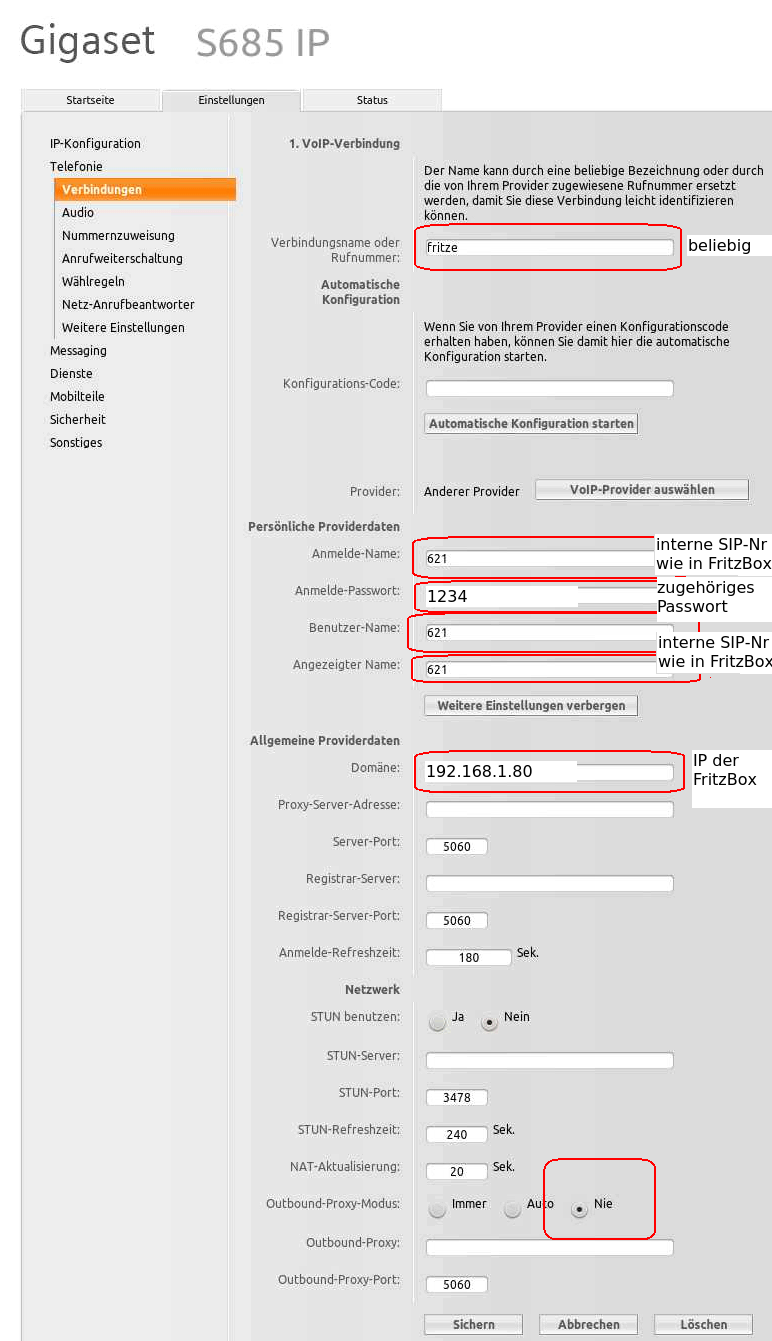
\includegraphics[width=.8\hsize]{./images/voip-client-s685ip-01.png}
\end{center}
\caption[Konfiguration eines SIP-Accounts in der DECT-Basis Siemens S685IP]
{\label{voip-client-nexus5}Konfiguration eines SIP-Accounts in der DECT-Basis Siemens S685IP. Quelle:Autor}
\end{figure}

Wenn man den Account wie im Bild angelegt hat, erscheint oft direkt eine Fehlermeldung ''Anmeldung nicht möglich`` oder ähnlich klingend.
Davon sollte man sich nicht verunsichern lassen, die DECT-Basis regiert generell ser träge im Bezug auf die Weboberfläche und braucht daher
auch zur Anmeldung an der FritzBox einige Sekunden, also Geduld. Weiterhin sollte man noch die EInstellungen wie im folgenden Bild anpassen, falls
die Registrierung an der FritzBox dauerhaft fehlschlägt.

\begin{figure}[H]
\begin{center}
%\includegraphics[width=.5\hsize]{./images/informationweek-virtualizationbycathegory.png}
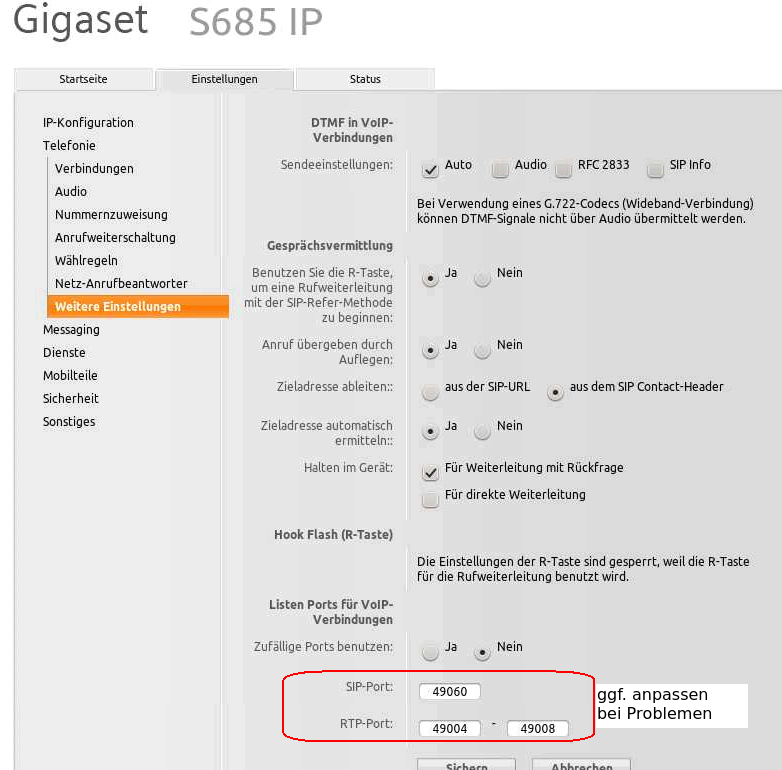
\includegraphics[width=.8\hsize]{./images/voip-client-s685ip-02.png}
\end{center}
\caption[Konfiguration eines SIP-Accounts in der DECT-Basis Siemens S685IP - weitere Einstellungen.]
{\label{voip-client-nexus5}Konfiguration eines SIP-Accounts in der DECT-Basis Siemens S685IP - weitere Einstellungen. Quelle:Autor}
\end{figure}

Anmerkung zum S685IP ansich: auch wenn die Weboberfläche einiges an Geduld erfordert, so hat sich das S685IP in 5 Jahren Benutzung als sehr zuverlässig 
erwiesen und die Investition von damals 130 Euro kann als gerechtfertigt angesehen werden. Auch die Reichweite ist im Vergleich zum DECT-Teil einer FritzBox
7270 mindestens doppelt so hoch. Wenn man nicht soviel Geld ausgeben möchte, kann man sich beim Auktionshaus seiner Wahl auch ein T-Home Sinus-501-V holen, dass
ist im Prinzip eine umgelabelte S6885IP. Einziger Unterschied zur ''echten`` S685IP ist das die Weboberfläche in magenta gehalten ist und der Festnetzanschluss (analog)
weggelassen wurde.

\subsection{Cisco 7960}
Das Cisco 7960 ist ein älteres, aber qualitativ hochweriges Systemtelefon mit, welches standardmäßig mit Ciscos proprietärem SCCP-Protokoll daher kommt. Da meines Wissens nur die Cisco Call Manager dieses Protokoll 
sprechen, muss dem Telefon erstmal eine SIP-Firmware untergeschoben werden. Das 7960 in unserem Beispiel soll die MAC-Adresse 00:12:34:56:78:ab haben, damit das Prinzip klar wird. Die echte Adresse steht hinten auf dem Telefon auf 
einem Aufkleber. 

Wir haben nun also 2 Schritte vor uns. Erstens müssen wir die Konfigurationsdateien anlegen, damit diese für unser Setup passen. Zweitens müssen wir die SIP-Firmwaredateien sowie die erstellten Konfigurationsdateien 
auf das Telefon befördern, damit dieses mit der FritzBox arbeiten kann.

\subsubsection{Konfigurationsdateien für das Cisco 7960 erstellen}

Die aktuellste SIP-Firmware für das 7960 liefert Cisco in einem Zip-File namens P0S3-8-12-00.zip welches man über eine kostenlose Registrierung
direkt bei Cisco oder durch geschicktes googlen finden kann. Wenn man die Zip-Datei entpackt erhält man folgende Dateien:
\begin{itemize}
 \item OS79XX.TXT
 \item P003-8-12-00.bin
 \item P003-8-12-00.sbn
 \item P003-8-12-00.loads
 \item P003-8-12-00.sb2
\end{itemize}

Neben diesen Dateien müssen wir jetzt noch weitere Dateien in diesem Verzeichnis anlegen:

\begin{lstlisting}[caption={SIPDefault.cnf},label=lst:7960sipdefaultcnf]
image_version: P0S3-8-12-00
proxy1_address: "192.168.1.80"   ; Can be dotted IP or FQDN
proxy2_address: ""              ; Can be dotted IP or FQDN
proxy3_address: ""              ; Can be dotted IP or FQDN
proxy4_address: ""              ; Can be dotted IP or FQDN
proxy5_address: ""              ; Can be dotted IP or FQDN
proxy6_address: ""              ; Can be dotted IP or FQDN
proxy_register: 1
messages_uri:   "1"
phone_password: "1234" ; Limited to 31 characters (Default - cisco)
sntp_mode: unicast
sntp_server: "192.168.1.1" 
time_zone: "CET" ; assuming you are in central europe
time_format_24hr: 1 ; to show the time in 24hour format
date_format: "D/M/Y"  ; format you would like the date in
\end{lstlisting}

\begin{lstlisting}[caption={XMLDefault.cnf.xml},label=lst:7960sipdefaultcnf]
<Default>
  <callManagerGroup>
     <members>
        <member priority="0">
           <callManager>
              <ports>
                 <ethernetPhonePort>2000</ethernetPhonePort>
                 <mgcpPorts>
                    <listen>2427</listen>
                    <keepAlive>2428</keepAlive>
                 </mgcpPorts>
              </ports>
              <processNodeName></processNodeName>
           </callManager>
        </member>
     </members>
  </callManagerGroup>
  <loadInformation7  model="Cisco 7960">P0S3-8-12-00</loadInformation7>
 <authenticationURL></authenticationURL>
 <directoryURL></directoryURL>
 <idleURL></idleURL>
 <informationURL></informationURL>
 <messagesURL></messagesURL>
 <servicesURL></servicesURL>
</Default>
\end{lstlisting}

In den folgenden beiden Konfigurationsdateien besteht ein Teil des Dateinamens aus der MAC-Adresse des Telefons, in unserem Beispiel lautet die MAC-Adresse des Telefons 00:12:34:56:78:ab.
Die beiden noch fehlenden Dateien für dieses Telefon heißen somit:
\begin{itemize}
 \item SEP\textbf{0012345678AB}.cnf.xml
 \item SIP\textbf{0012345678AB}.cnf
\end{itemize}
und haben folgenden Inhalt:

\begin{lstlisting}[caption={SEP\textbf{0012345678AB}.cnf.xml},label=lst:7960sep0012345678abcnfxml]
<device>
<loadInformation model="IP Phone 7960">P0S3-8-12-00</loadInformation>
</device>
\end{lstlisting}

\begin{lstlisting}[caption={SIP\textbf{0012345678AB}.cnf},label=lst:7960sip0012345678abcnf]
image_version: P0S3-8-12-00
line1_name: 622
line1_authname: "622"
line1_shortname: "622" ; displayed on the phones softkey
line1_password: "1234"
line1_displayname: "622"; the caller id
proxy1_port: 5060
proxy1_address: 192.168.1.80
# Phone Label (Text desired to be displayed in upper right corner)
phone_label: "Werkstatt " ; add a space at the end, looks neater
phone_password: "1234" ; Limited to 31 characters (Default - cisco)
user_info: none
telnet_level: 2
logo_url: "http://192.168.1.203/cisco/asterisk-tux.bmp"
\end{lstlisting}

Nun sollten sich in dem Verzeichnis die folgenden Dateien befinden:
\begin{itemize}
 \item OS79XX.TXT  
 \item P003-8-12-00.bin  
 \item P003-8-12-00.sbn  
 \item P0S3-8-12-00.loads
 \item P0S3-8-12-00.sb2
 \item SEP0012345678AB.cnf.xml
 \item SIP0012345678AB.cnf
 \item SIPDefault.cnf
\end{itemize}
Wenn alles klappt sollte sich das Telefon nach dem Update in einer Minimalkonfiguration befinden, also sich an der FritzBox anmelden und ein- und ausgehende Gespräche möglich sein.

\subsubsection{Konfigurationsdateien und TFTP-Server für Cisco 7960 vorbereiten}
Um die Dateien aus dem vorherigen Kaptiel auf das Telefon zu bekommen, muss man einen TFTP-Server installieren. 
Ich habe hier einen Ubuntu-Server verwendet auf dem ich den atftp installiert habe:

\lstset{
	language=BASH,
	keywordstyle=\bfseries\ttfamily\color[rgb]{0,0,1},
	identifierstyle=\ttfamily,
	commentstyle=\color[rgb]{0.133,0.545,0.133},
	stringstyle=\ttfamily\color[rgb]{0.627,0.126,0.941},
	showstringspaces=false,
	basicstyle=\scriptsize,
	tabsize=1,
	numbers=left,                    % where to put the line-numbers; possible values are (none, left, right)
	numbersep=5pt,                   % how far the line-numbers are from the code
	numberstyle=\tiny\color{gray}, % the style that is used for the line-numbers
	breaklines=true,	%automatischer Zeilenumbruch
	prebreak =\raisebox{0ex}[0ex][0ex]{\ensuremath{\hookleftarrow}},
	breakatwhitespace=false,
	aboveskip={1.5\baselineskip},
  	columns=fixed,
  	upquote=true,
  	extendedchars=true,
  	backgroundcolor=\color[rgb]{0.97,0.97,0.97},
}
\begin{lstlisting}[caption={Installation von atftp unter ubuntu},label=lst:atftpdinstall]
$ sudo apt-get update

$ sudo apt-get install atftpd
$ sudo apt-get remove xinetd

$ sudo mkdir /srv/tftp && sudo chown nobody.nogroup /srv/tftp
$ sudo touch /var/log/atftpd.log  && sudo chown nobody.nogroup /var/log/atftpd.log
\end{lstlisting}

Anschließend sind noch Modifikationen an der Konfigurationsdatei /etc/default/atftpdvon atftpd nötig, damit dieser selbstständig (ohne xinetd) und mit aktiviertem Logging
lauffähig ist. In der Logdatei kann man dann während des Updatevorgangs gut sehen ob und welche Telefone sich Dateien vom atftpd abholen.

\begin{lstlisting}[caption={atftpd-Konfigurationsdatei /etc/default/atftpd},label=lst:atftpdconfig]
USE_INETD=false
OPTIONS="--tftpd-timeout 300 --retry-timeout 5 --mcast-port 1758 --mcast-addr 239.239.239.0-255 --mcast-ttl 1 --maxthread 100 --verbose=6 --logfile /var/log/atftpd.log /srv/tftp"
\end{lstlisting}

Im letzten Schritt kopieren wir noch die im vorherigen Kapitel angelegten Dateien für das 7960 in das Stammverzeichnis des atftpd, nämlich /srv/tftp und passen die Berechtigungen an:
\begin{lstlisting}
$ cd /Verzeichnis/in/dem/die/Cisco7960/Dateien/liegen
$ sudo cp * /srv/tftp/
$ sudo chmod 660 /srv/tftp/*
$ sudo chown -R nobody.nogroup /srv/tftp
\end{lstlisting}

Am Ende sollte dieses Verzeichnis so aussehen:

\begin{lstlisting}
m@marlap01:~$ ls -hal /srv/tftp/
insgesamt 1,0M
drwxr-xr-x 2 nobody nogroup 4,0K Jan 14 10:47 .
drwxr-xr-x 3 root   root    4,0K Jan 14 10:47 ..
-rw-rw---- 1 nobody nogroup   15 Jan 14 10:47 OS79XX.TXT
-rw-rw---- 1 nobody nogroup 128K Jan 14 10:47 P003-8-12-00.bin
-rw-rw---- 1 nobody nogroup 128K Jan 14 10:47 P003-8-12-00.sbn
-rw-rw---- 1 nobody nogroup  458 Jan 14 10:47 P0S3-8-12-00.loads
-rw-rw---- 1 nobody nogroup 739K Jan 14 10:47 P0S3-8-12-00.sb2
-rw-rw---- 1 nobody nogroup   89 Jan 14 10:47 SEP0012345678AB.cnf.xml
-rw-rw---- 1 nobody nogroup  535 Jan 14 10:47 SIP0012345678AB.cnf
-rw-rw---- 1 nobody nogroup  718 Jan 14 10:47 SIPDefault.cnf
m@marlap01:~$ 
\end{lstlisting}
Wenn man nun abschließend mittels

\begin{lstlisting}
$ sudo service atftpd restart
\end{lstlisting}

den atftpd noch dazu bringt die neue Konfiguration zu übernehmen, sollte der TFTP Server bereit sein. Nun ist noch dafür zu sorgen,
dass das Telefon weiß, unter welcher lokalen IP-Adresse es den TFTP-Server erreichen kann. Ich habe dazu einfach in meinem DHCP-Server
auf dem IGEL-Router als DHCP-Option die IP-Adresse des TFTP-Servers angegeben. Man kann wohl auch manuell im Telefon unter Netzwerkeinstellungen
eine IP-Adresse für den TFTP-Server angeben, dass hab ich jedoch selbst nicht ausprobiert.

\subsubsection{Cisco 7960 updaten}
Da nun alles vorbereitet ist holen wir zum Radikalschlag aus: Wir müssen die Firmware des Telefons komplett platt machen. In Folge dessen versucht das
Telefon dann per TFTP eine neue Firmware und Konfiguration vom angegebenen TFTP-Server zu laden und bekommt diesmal die SIP-Firmware untergeschoben.

Um den Firmware-Reset durchzuführen müssen wir das 7960 vom Strom trennen. Dann wird der Strom wieder verbunden und direkt danach die Rautetaste \# gedrückt gehalten.
Wir halten \# solange gedrückt, bis die drei Tasten rechts unten abwechselnd anfangen zu blinken. Indem wir jetzt nacheinander die Tasten 1 2 3 4 5 6 7 8 9 * 0 \# drücken starten wir den
Firmwarereset mit anschließendem Update. Zur Fehlerdiagnose sollte man die LOG-Datei des TFTP-Servers beobachten. Ich hatte anfangs das Problem, das das Telefon die IP des TFTP-Servers
nicht übernommen hat und somit die Dateien nicht laden konnte. 

Nun ist etwas Geduld gefragt. Nachdem das Telefon im Verlauf des Updatevorgangs mehrmals neu gestartet hat, sollte es sich mit der neuen Konfiguration an der FritzBox anmelden und kann 
verwendet werden. Sollte irgendwas schief gehen bitte folgende Sachen überprüfen:

\begin{itemize}
 \item stimmt die MAC-Adresse mit den Konfigurationsdateien überein ?
 \item holt sich das Telefon vom DHCP-Server die vorgesehene Adresse ? (ping)
 \item holt das Telefon Dateien vom TFTP Server ? (LOG-Dateien prüfen: tail -f /var/log/atftp.log )
 \item ist die IP-Adresse für die FritzBox richtig in den Konfigurationsdateien ausgewiesen ?
 \item stimmen die SIP-Anmeldedaten überein (vergleiche FritzBox-Telefoniegrät und Benutzername/Passwort in Konfigurationsdatei für das Telefon) 
\end{itemize}


\subsection{Cisco 7961}
Die Konfiguration für das Cisco 7961 ist im prinzip sehr ähnlich. Wir gehen wieder in zwei Schritten vor. Erstens erstellen wir die individuellen Konfigurationsdateien für unser 
Beispieltelefon Cisco 7961 mit der beispielhaften MAC-Adresse 00:12:34:56:78:de. Im zweiten Schritt bemühen wir dann wieder die Webseite von Cisco um an die aktuelleste SIP-Firmware für unser
Cisco 7961 zu kommen.

\subsubsection{Konfigurationsdateien für das Cisco 7961 erstellen}
Die aktuellste SIP-Firmware für das Cisco 7961 ist im Moment in der Datei cmterm-7941\_7961-sip.9-4-2SR1-1.zip\footnote{\url{https://software.cisco.com/download/release.html?mdfid=279251499\&flowid=46206\&softwareid=282074288\&release=9.4(2)SR1\&relind=AVAILABLE\&rellifecycle=\&reltype=latest}} enthalten. Nach dem entpacken sehen wir folgende Dateien:

\begin{itemize}
 \item apps41.9-4-2ES9.sbn  
 \item cnu41.9-4-2ES9.sbn
 \item cvm41sip.9-4-2ES9.sbn
 \item dsp41.9-4-2ES9.sbn
 \item jar41sip.9-4-2ES9.sbn
 \item SIP41.9-4-2SR1-1S.loads
 \item term41.default.loads
 \item term61.default.loads
\end{itemize}

Zusätzlich legen wir jetzt noch die folgenden Dateien an:
\lstset{
	language=BASH,
	keywordstyle=\bfseries\ttfamily\color[rgb]{0,0,1},
	identifierstyle=\ttfamily,
	commentstyle=\color[rgb]{0.133,0.545,0.133},
	stringstyle=\ttfamily\color[rgb]{0.627,0.126,0.941},
	showstringspaces=false,
	basicstyle=\scriptsize,
	tabsize=1,
	numbers=left,                    % where to put the line-numbers; possible values are (none, left, right)
	numbersep=5pt,                   % how far the line-numbers are from the code
	numberstyle=\tiny\color{gray}, % the style that is used for the line-numbers
	breaklines=true,	%automatischer Zeilenumbruch
	prebreak =\raisebox{0ex}[0ex][0ex]{\ensuremath{\hookleftarrow}},
	breakatwhitespace=false,
	aboveskip={1.5\baselineskip},
  	columns=fixed,
  	upquote=true,
  	extendedchars=true,
  	backgroundcolor=\color[rgb]{0.97,0.97,0.97},
}
\begin{lstlisting}[caption={dialplan.xml},label=lst:dialplanxml]
<DIALTEMPLATE>
  <TEMPLATE MATCH="*" Timeout="5" />
</DIALTEMPLATE>
\end{lstlisting}    
                
Die folgende XML-Datei enthält alle wesentlichen Einstellungen für das Telefon, welches die mit dem Dateinamen korrespondierende MAC-Adresse hat. Unter anderem wird in dieser Datei
auch der Telefonname in Zeile 145 festgelegt, hierbei keine Leerzeichen verwenden, da das Telefon sonst die gesamte Konfigurationsdatei verwirft und in den Status ''unprovisioniert über geht``.
\begin{lstlisting}[caption={SEP\textbf{0012345678DE}.cnf.xml}, label=lst:cisco7961sep0012345678decnfxml]               
<?xml version="1.0" encoding="UTF-8"?>
<device>
  <deviceProtocol>SIP</deviceProtocol>
  <sshUserId>admin</sshUserId>
  <sshPassword>1234</sshPassword>
  <devicePool>
    <dateTimeSetting>
      <dateTemplate>D.M.YY</dateTemplate>
      <timeZone>Central Europe Standard/Daylight Time</timeZone>
	<ntps>
	  <ntp>
	    <name>192.168.1.1</name>
	    <ntpMode>Unicast</ntpMode>
	  </ntp>
	</ntps>
      </dateTimeSetting>
      <callManagerGroup>
	<members>
	  <member priority="0">
	    <callManager>
	      <ports>
		<ethernetPhonePort>2000</ethernetPhonePort>
		<sipPort>5060</sipPort>
		<securedSipPort>5061</securedSipPort>
	      </ports>
	    <processNodeName>192.168.1.80</processNodeName>
	  </callManager>
	</member>
      </members>
    </callManagerGroup>
  </devicePool>
  <commonProfile>
    <phonePassword></phonePassword>
    <backgroundImageAccess>true</backgroundImageAccess>
    <callLogBlfEnabled>2</callLogBlfEnabled>
  </commonProfile>
  <loadInformation>SIP41.9-4-2SR1-1S</loadInformation>
  <vendorConfig>
     <disableSpeaker>false</disableSpeaker>
     <disableSpeakerAndHeadset>false</disableSpeakerAndHeadset>
     <pcPort>1</pcPort>
     <settingsAccess>1</settingsAccess>
     <garp>0</garp>
     <voiceVlanAccess>0</voiceVlanAccess>
     <videoCapability>0</videoCapability>
     <autoSelectLineEnable>0</autoSelectLineEnable>
     <sshAccess>0</sshAccess>
     <sshPort>22</sshPort>
     <webAccess>1</webAccess>
     <spanToPCPort>1</spanToPCPort>
     <loggingDisplay>1</loggingDisplay>
     <loadServer></loadServer>
     <daysDisplayNotActive></daysDisplayNotActive>
     <displayOnTime>03:00</displayOnTime>
     <displayOnDuration>00:01</displayOnDuration>
     <displayIdleTimeout>00:05</displayIdleTimeout>
     <displayOnWhenIncomingCall>1</displayOnWhenIncomingCall>
  </vendorConfig>
  <deviceSecurityMode>1</deviceSecurityMode>
  <authenticationURL>http://192.168.1.80/ciscoauth.php</authenticationURL>
  <directoryURL>http://192.168.1.80/directory.php</directoryURL>
  <idleURL></idleURL>
  <informationURL></informationURL>
  <messagesURL></messagesURL>
  <proxyServerURL></proxyServerURL>
  <servicesURL></servicesURL>
  <dscpForSCCPPhoneConfig>96</dscpForSCCPPhoneConfig>
  <dscpForSCCPPhoneServices>0</dscpForSCCPPhoneServices>
  <dscpForCm2Dvce>96</dscpForCm2Dvce>
  <transportLayerProtocol>2</transportLayerProtocol>
  <capfAuthMode>0</capfAuthMode>
  <capfList>
     <capf>
        <phonePort>3804</phonePort>
     </capf>
  </capfList>
  <certHash></certHash>
  <encrConfig>false</encrConfig>
   <sipProfile>
     <sipProxies>
        <backupProxy></backupProxy>
        <backupProxyPort></backupProxyPort>
        <emergencyProxy></emergencyProxy>
        <emergencyProxyPort></emergencyProxyPort>
        <outboundProxy></outboundProxy>
        <outboundProxyPort></outboundProxyPort>
        <registerWithProxy>true</registerWithProxy>
     </sipProxies>
     <sipCallFeatures>
        <cnfJoinEnabled>true</cnfJoinEnabled>
        <callForwardURI>x--serviceuri-cfwdall</callForwardURI>
        <callPickupURI>x-cisco-serviceuri-pickup</callPickupURI>
        <callPickupListURI>x-cisco-serviceuri-opickup</callPickupListURI>
        <callPickupGroupURI>x-cisco-serviceuri-gpickup</callPickupGroupURI>
        <meetMeServiceURI>x-cisco-serviceuri-meetme</meetMeServiceURI>
        <abbreviatedDialURI>x-cisco-serviceuri-abbrdial</abbreviatedDialURI>
        <rfc2543Hold>false</rfc2543Hold>
        <callHoldRingback>2</callHoldRingback>
        <localCfwdEnable>true</localCfwdEnable>
        <semiAttendedTransfer>true</semiAttendedTransfer>
        <anonymousCallBlock>2</anonymousCallBlock>
        <callerIdBlocking>2</callerIdBlocking>
        <dndControl>0</dndControl>
        <remoteCcEnable>true</remoteCcEnable>
     </sipCallFeatures>
     <sipStack>
        <sipInviteRetx>6</sipInviteRetx>
        <sipRetx>10</sipRetx>
        <timerInviteExpires>180</timerInviteExpires>
        <timerRegisterExpires>3600</timerRegisterExpires>
        <timerRegisterDelta>5</timerRegisterDelta>
        <timerKeepAliveExpires>120</timerKeepAliveExpires>
        <timerSubscribeExpires>120</timerSubscribeExpires>
        <timerSubscribeDelta>5</timerSubscribeDelta>
        <timerT1>500</timerT1>
        <timerT2>4000</timerT2>
        <maxRedirects>70</maxRedirects>
        <remotePartyID>false</remotePartyID>
        <userInfo>None</userInfo>
     </sipStack>
     <autoAnswerTimer>1</autoAnswerTimer>
     <autoAnswerAltBehavior>false</autoAnswerAltBehavior>
     <autoAnswerOverride>true</autoAnswerOverride>
     <transferOnhookEnabled>false</transferOnhookEnabled>
     <enableVad>false</enableVad>
     <preferredCodec>g711alaw</preferredCodec>
     <dtmfAvtPayload>101</dtmfAvtPayload>
     <dtmfDbLevel>3</dtmfDbLevel>
     <dtmfOutofBand>avt</dtmfOutofBand>
     <alwaysUsePrimeLine>false</alwaysUsePrimeLine>
     <alwaysUsePrimeLineVoiceMail>false</alwaysUsePrimeLineVoiceMail>
     <kpml>3</kpml>
     <natEnabled>false</natEnabled>
     <natAddress></natAddress>
     <stutterMsgWaiting>0</stutterMsgWaiting>
     <callStats>false</callStats>
     <silentPeriodBetweenCallWaitingBursts>10</silentPeriodBetweenCallWaitingBursts>
     <disableLocalSpeedDialConfig>false</disableLocalSpeedDialConfig>
     <startMediaPort>16384</startMediaPort>
     <stopMediaPort>32766</stopMediaPort>
     <voipControlPort>5060</voipControlPort>
     <dscpForAudio>184</dscpForAudio>
     <ringSettingBusyStationPolicy>0</ringSettingBusyStationPolicy>
     <dialTemplate>dialplan.xml</dialTemplate>
     <phoneLabel>Schlafzimmer</phoneLabel>
     <sipLines>
        <line button="1">
           <featureID>9</featureID>
           <featureLabel>623</featureLabel>
           <name>623</name>
           <displayName>623</displayName>
           <contact>623</contact>
           <proxy>USECALLMANAGER</proxy>
           <port>5060</port>
           <autoAnswer>
              <autoAnswerEnabled>2</autoAnswerEnabled>
           </autoAnswer>
           <callWaiting>3</callWaiting>
           <authName>624</authName>
           <authPassword>1234</authPassword>
           <sharedLine>false</sharedLine>
           <messageWaitingLampPolicy>1</messageWaitingLampPolicy>
           <messagesNumber>*97</messagesNumber>
           <ringSettingIdle>4</ringSettingIdle>
           <ringSettingActive>5</ringSettingActive>
           <forwardCallInfoDisplay>
              <callerName>true</callerName>
              <callerNumber>true</callerNumber>
              <redirectedNumber>false</redirectedNumber>
              <dialedNumber>true</dialedNumber>
           </forwardCallInfoDisplay>
        </line>
        <line button="2">
           <featureID>2</featureID>
           <featureLabel>Werkstatt</featureLabel>
           <speedDialNumber>**622</speedDialNumber>
        </line>
        <line button="6">
           <featureID>2</featureID>
           <featureLabel>Mobilteile</featureLabel>
           <speedDialNumber>**621</speedDialNumber>
        </line>
     </sipLines>
  </sipProfile>
</device>
\end{lstlisting}

Zum Schluss ergänzen wir die aus dem letzten Kapitel bekannte XMLDefault.cnf.xml um einen Eintrag, der allen anfragenden Cisco 7961 mitteilt welche Firmware sie laden sollen.
Wenn du das Kapitel Cisco 7960 übersprungen hast kannst du diese Datei trotzdem wie nachfolgend gezeigt anlegen:

\begin{lstlisting}[caption={XMLDefault.cnf.xml für Cisco 7960 und 7961 gültig}, label=lst:xmldefaultcnfcml79607961]    
<Default>
  <callManagerGroup>
    <members>
      <member priority="0">
	<callManager>
	  <ports>
	    <ethernetPhonePort>2000</ethernetPhonePort>
	      <mgcpPorts>
		<listen>2427</listen>
		<keepAlive>2428</keepAlive>
	      </mgcpPorts>
	    </ports>
	    <processNodeName></processNodeName>
	</callManager>
      </member>
    </members>
  </callManagerGroup>
  <loadInformation7  model="Cisco 7960">P0S3-8-12-00</loadInformation7>
  <loadInformation30018  model="Cisco 7961">SIP41.9-4-2SR1-1S</loadInformation30018>
  <loadInformation308  model="Cisco 7961G-GE">SIP41.9-4-2SR1-1S</loadInformation308>
  <authenticationURL></authenticationURL>
  <directoryURL></directoryURL>
  <idleURL></idleURL>
  <informationURL></informationURL>
  <messagesURL></messagesURL>
  <servicesURL></servicesURL>
</Default>
\end{lstlisting}

Nachdem diese 3 Dateien erstellt wurden, sollten wir nun insgesamt diese Dateien alle in unserem Verzeichnis sehen:
\begin{itemize}
 \item apps41.9-4-2ES9.sbn  
 \item cnu41.9-4-2ES9.sbn
 \item cvm41sip.9-4-2ES9.sbn
 \item dialplan.xml
 \item dsp41.9-4-2ES9.sbn
 \item jar41sip.9-4-2ES9.sbn
 \item SEP\textbf{0012345678DE}.cnf.xml
 \item SIP41.9-4-2SR1-1S.loads
 \item term41.default.loads
 \item term61.default.loads
 \item XMLDefault.cnf.xml
\end{itemize}
Wenn dies der Fall ist, dann bitte im nächsten Kapitel fortfahren, sonst die letzten Schritte nochmal überprüfen !

\subsubsection{Konfigurationsdateien und TFTP-Server für Cisco 7961 vorbereiten}
Da wir den TFTP-Server ja im Kapitel für das Cisco 7960 vorbereitet haben, brauchen wir nun nur die Dateien in das Verzeichnes /srv/tftp/ des TFTP-Servers kopieren.
Da über die XMLDefault.cnf.xml definiert ist, welche Telefonmodelle welche Firmware beziehen sollen, kann man problemlos die Firmwaredateien beider Telefonmodelle auf 
dem TFTP-Server belassen. Leser, welche das Kapitel Cisco 7960 übersprungen haben, können bei Bedarf im Kapitel \textbf{Konfigurationsdateien und TFTP-Server für Cisco 7960 vorbereiten}
nachlesen, wie man einen atftpd-Server unter Ubuntu so installiert und konfiguriert, das die Cisco's von dort die Firmwaredateien beziehen können.

\subsubsection{Cisco 7961 updaten}
Wie auch beim Cisco 7960 gehen wir nun beim Cisco 7961 vor um die derzeitig auf dem Gerät befindliche Firmware zu löschen und die neue SIP-Firmware zu installieren:

\begin{itemize}
 \item Cisco 7961 vom Strom trennen und kurz warten 
 \item Cisco 7961 wieder mit STrom versorgen und direkt danach die Raute-Taste \# gedrückhalt, solange bis die Line-Tasten rechts neben dem Bildschirm anfangen zu blinken
 \item nun \# Taste loslassen und nach einander die Tasten 1 2 3 4 5 6 7 8 9 * 0 \# drücken, Line-Tasten sollten innerhalb von 3 Sekunden aufhören zu blinken
 \item \textbf{NUN ABWARTEN UND GEDULD HABEN} - das Telefon braucht (dank Java) ca. eine halbe Stunde um das Update durchzuführen und startet währenddessen mehrmals neu. 
 \item wenn der Updatevorgang abgeschlossen ist, sollte sich das Telefon mit der FritzBox verbinden und benutzbar sein, d.h. abgehende und ankommende Anrufe intern und auch extern
\end{itemize}

\subsection{Cisco 7962}
Über das Auktionshaus meiner Wahl bin ich noch an 5 gebrauchte Cisco 7962 gekommen. Die 7962 scheinen im Gegensatz zu den Vorgängern jedoch von einem ärgerlichen Problem betroffen zu sein:
ich habe bei 4 von 5 der 7962 das Problem, dass diese nicht korrekt booten. Sobald man diese mit Energie versorgt, beginnt die Freisprechtaste grün zu leuchten und das wars.
An diesem Zustand ändert sich auch nach Stunden nichts. Alles was ich im Internet dazu gefunden habe, ist der Hinweis bei Cisco einen RMA-Fall zu eröffnen, was für mich als Gebrauchtwarenkäufer
natürlich nicht möglich ist. Bisher habe ich noch keine Möglichkeit gefunden das Problem zu fixen. Empfehlung: Modelle der Serien 79*1 oder 79*0 kaufen, falls möglich.

Das einzige 7962 mit intakten Bootloader konnten ich mit einem Vorgehen analog zum 7961 integrieren.

\subsubsection{Konfigurationsdateien und TFTP-Server für Cisco 7962 vorbereiten}
Da wir den TFTP-Server ja im Kapitel für das Cisco 7960 vorbereitet haben, brauchen wir nun nur die SIP-Firmware-Dateien in das Verzeichnes /srv/tftp/ des TFTP-Servers kopieren.
Da über die XMLDefault.cnf.xml definiert ist, welche Telefonmodelle welche Firmware beziehen sollen, kann man problemlos die Firmwaredateien der verschiedenen Telefonmodelle auf 
dem TFTP-Server belassen. Leser, welche das Kapitel Cisco 7960 übersprungen haben, können bei Bedarf im Kapitel \textbf{Konfigurationsdateien und TFTP-Server für Cisco 7960 vorbereiten}
nachlesen, wie man einen atftpd-Server unter Ubuntu so installiert und konfiguriert, das die Cisco's von dort die Firmwaredateien beziehen können. Die aktuelle SIP-Firmware für 7962 Telefone
kann man mit einem kostenlosen Account unter \footnote{\url{http://www.cisco.com/c/en/us/td/docs/voice\_ip\_comm/cuipph/7900\_series/firmware/9\_4\_2SR2/english/releasenotes/P790\_BK\_C7078DFD\_00\_cisco-unified-ip-phone-7900.html}} als Zip-Datei mit dem Namen \textbf{cmterm-7942\_7962-sip.9-4-2SR1-1.zip} runterladen.

Die XMLDefault.cnf.xml sieht für ein gemischtes Setup aus 7960, 7961 und 7962 so aus:
\begin{lstlisting}[caption={XMLDefault.cnf.xml für Cisco 7960, 7961 und 7962 gültig}, label=lst:xmldefaultcnfcml796079617962]    
<Default>
  <callManagerGroup>
    <members>
      <member priority="0">
	<callManager>
	  <ports>
	    <ethernetPhonePort>2000</ethernetPhonePort>
	      <mgcpPorts>
		<listen>2427</listen>
		<keepAlive>2428</keepAlive>
	      </mgcpPorts>
	    </ports>
	    <processNodeName></processNodeName>
	</callManager>
      </member>
    </members>
  </callManagerGroup>
  <loadInformation7  model="Cisco 7960">P0S3-8-12-00</loadInformation7>
  <loadInformation30018  model="Cisco 7961">SIP41.9-4-2SR1-1S</loadInformation30018>
  <loadInformation308  model="Cisco 7961G-GE">SIP41.9-4-2SR1-1S</loadInformation308>
  <loadInformation30018  model="Cisco 7962">SIP42.9-4-2SR1-1S</loadInformation30018> 
  <loadInformation308  model="Cisco 7962G-GE">SIP42.9-4-2SR1-1S</loadInformation308> 
  <authenticationURL></authenticationURL>
  <directoryURL></directoryURL>
  <idleURL></idleURL>
  <informationURL></informationURL>
  <messagesURL></messagesURL>
  <servicesURL></servicesURL>
</Default>
\end{lstlisting}

Die SEP<mac-adresse>.xml kann von der Vorlage für die 7961 Telefone übernommen werden. Am Ende sieht das Datenverzeichnis meines TFTP-Servers so aus, damit sowohl 7960, wie auch 
7961 und 7962 provisioniert werden können:

\begin{figure}[H]
\begin{center}
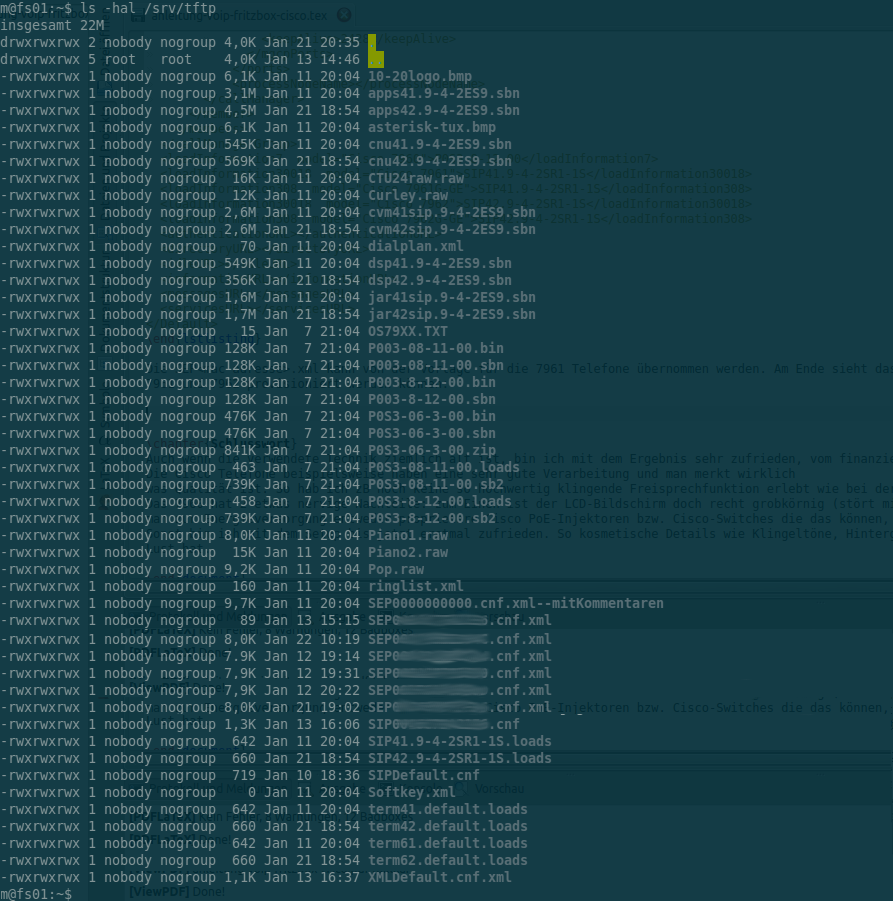
\includegraphics[width=1\hsize]{./images/atftpd-cisco7960-7961-7962.png}
\end{center}
\caption[TFTP-Server Datenverzeichnis für ein vollständiges 7960/7961/7962 Deployment.]
{\label{atftpd-7960-7961-7962}TFTP-Server Datenverzeichnis für ein vollständiges 7960/7961/7962 Deployment. Quelle: Autor}
\end{figure}

\chapter{Schlusswort}
Auch wenn die verwendete Technik ziemlich alt ist, bin ich mit dem Ergebnis sehr zufrieden, vom finanziellen Aufwand her wie auch von der Zuverlässigkeit und der Qualität. 
Die Cisco Telefone beispielsweise haben eine sehr gute Verarbeitung und man merkt wirklich
was Qualität ist. So hab ich zB noch keine so hochwertig klingende Freisprechfunktion erlebt wie bei der 796* Serie. Meiner Meinung nach nehmen sich die einzelnen Modelle der 796*er Serie auch nicht viel.
Das 7960 hat 2 etwas nervige Nachteile: zum Einen ist der LCD-Bildschirm doch recht grobkörnig (stört mich weniger) und das 7960 unterstützt noch kein PoE nach 802.3af. Somit braucht
man zur Energieversorgung entweder proprietäre Cisco PoE-Injektoren bzw. Cisco-Switches die das können, oder eben ein 48V-Netzteil - da hat man dann aber wieder 2 Kabel zum Telefon.
Sonst bin ich mit dem Setup bis jetzt erstmal zufrieden. So kosmetische Details wie Klingeltöne, Hintergrundbilder etc. hab ich jetzt mal außen vor gelassen, dass kann jeder machen wie er/sie 
Lust hat. Von Erwerb gebrauchter 7962 ohne Garantie rate ich derzeit ab, da man nicht weiss ob man Geräte mit intaktem Bootloader erhält. 7962-Telefone mit korruptem Bootloader kann man nach meinem
derzeitigen Kenntnisstand nur als Ersatzteilspender verwenden. 

\end{document}
